\section{Lecture 6: Heisenberg Uncertainty Continued, Schrodinger's Equation}

In the quantum theory of an atom, electrons have defined energy levels. 

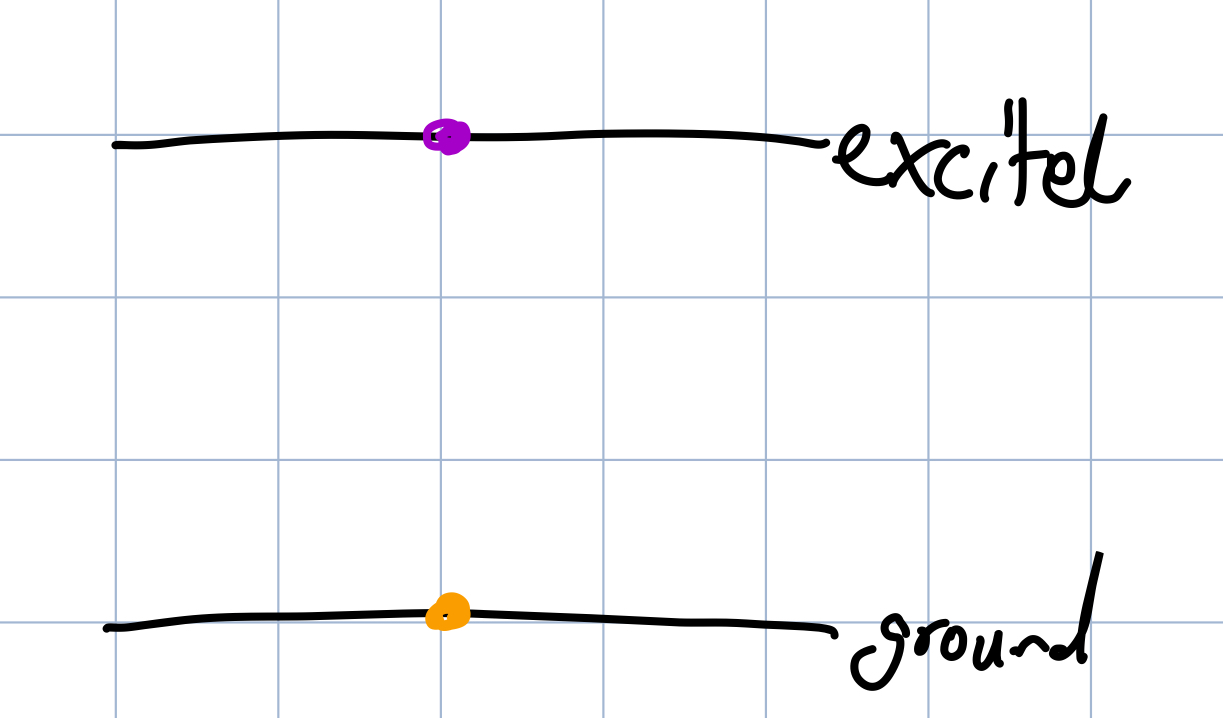
\includegraphics[width=300px]{energieslevs.jpeg}

Consider an electron in the ground state--it can stay
there for basically an infinite amount of time. When an electron is in the excited state, then
it will drop down at some indeterminate time. If you average this together, you get a half life decay like this:

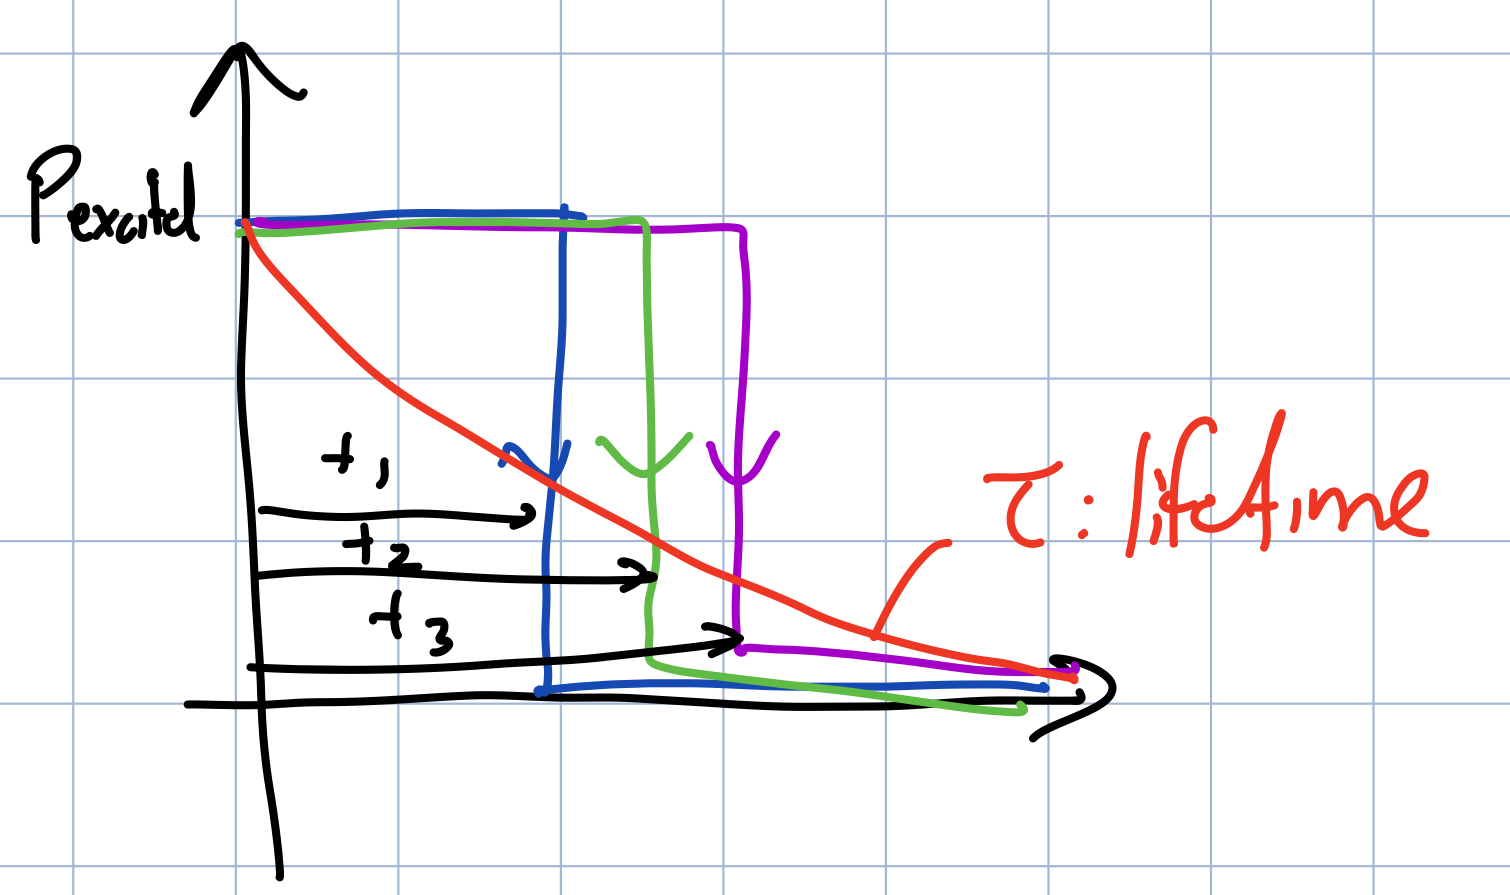
\includegraphics[width=300px]{drops.jpeg}

Because this is really a probability distribution, you actually see a small band of frequencies. The uncertainty is:

\[ \Delta E = \frac{\hbar}{\tau} \]

The diagram now more accurately looks like this:

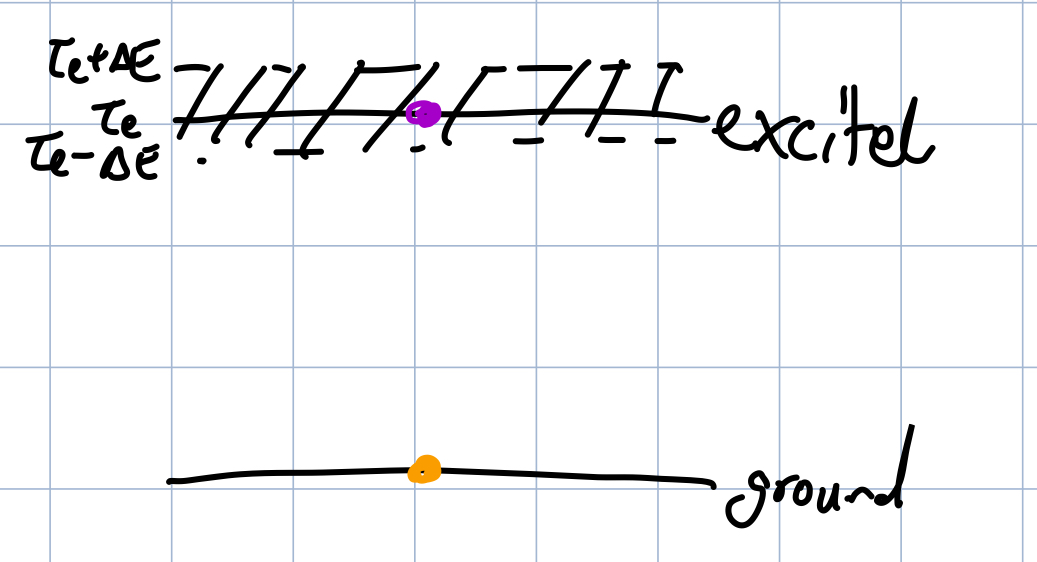
\includegraphics[width=300px]{newlevs.jpeg}

and the photon emission spectrum looks like this.

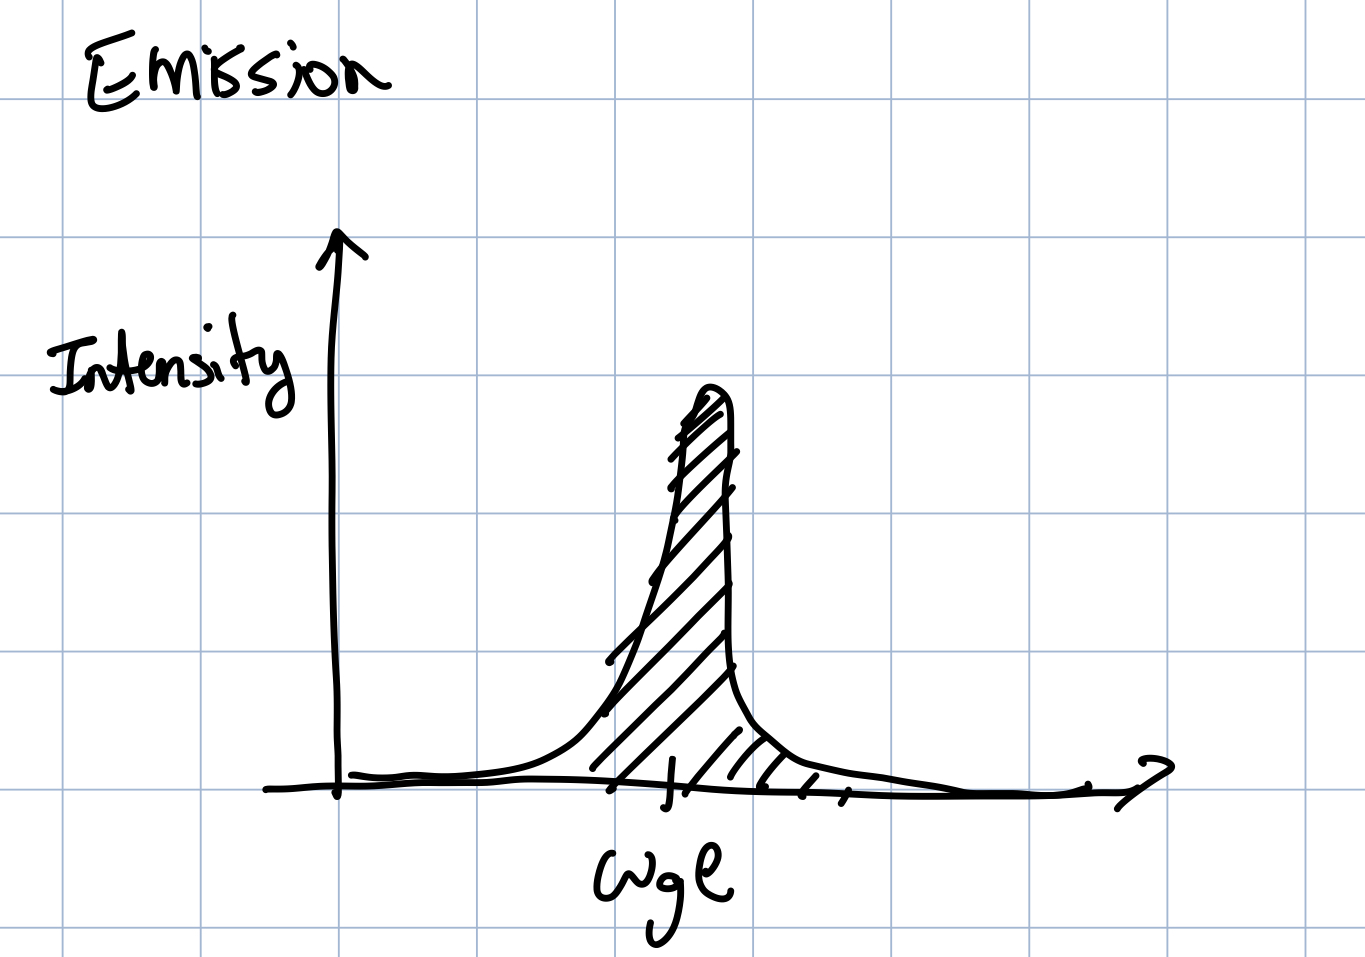
\includegraphics[width=300px]{spectrums.jpeg}

Imagine now a flourescent tube. Once you excited an atom on the edge of the tube, how do the atoms in the middle shine?
Well, the atoms emit photons which are absorbed by neighboring atoms. However, by conservation of momentum, the atom must recoil backwards when emitting
a photon.

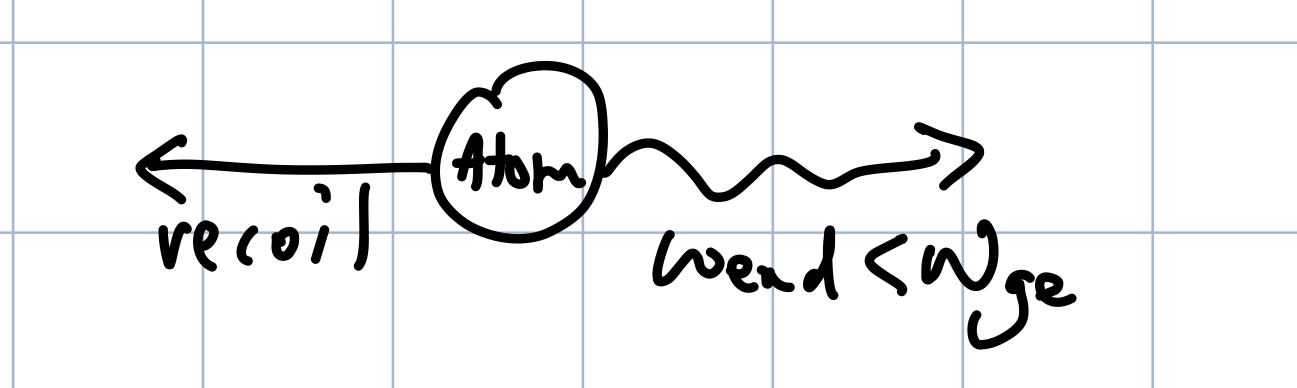
\includegraphics[width=300px]{atom_recoil.jpeg}

But since the atom spectra is actually a probability distribution and not pointwise, if the recoil is less than the line width, then you can get still get this resonance
with high probability. This is decidedly not true for nuclei and $\gamma$ rays, except if the entire lattice resonates, distributing the recoil over many particles. This is called the Mossbauer Effect,
and allows the bulb to work.

\subsection{Schrodinger's Wave Equation}
Now we want an equation that can give us the wave function. We want the following nice properties:
\begin{itemize}
    \item Linear (permits superposition, since superposition is done to waves)
    \item Should ``agree'' with classical physics
    \item There should be only one time derivative, because if there were two you would need two snapshots in time, i.e. causality reasons.
\end{itemize}

Suppose the wave function is:
\[ \Psi(x, t) = Ae^{i(p_x x - Et) \hbar} \]
Then we know that the energy is:
\[ E = \frac{p_x^2}{2m} \implies \omega = \frac{\hbar k^2}{2m} \]
which is called the dispersion relation for a free particle.
Furthermore, by the eigenfunction properties of the exponential:
\begin{align*}
    \partialderivative{\Psi(x, t)}{t} &= A(-i \omega)e^{i(kx - \omega t)} \\
    &= -i \omega \Psi = \frac{-i}{\hbar} E \Psi \\
    \partialderivative{^2 \Psi(x, t)}{x^2} &= - k^2 A e^{i(k x - \omega t)} \\
    &= \frac{-p_x^2}{\hbar^2} \Psi \\
    &= \frac{-2Em}{\hbar^2} \Psi
\end{align*}

Setting the $E$s equal yields:
\begin{theorem}[Schrodinger's Wave Equation - 1D Free Particle]
    The wave equation is
    \[ i \hbar \partialderivative{\Psi(x, t)}{t} = \frac{-\hbar^2}{2m} \partialderivative{^2\Psi(x, t)}{x^2} \]
    Where we can define operators:
    \[ \hat{E} = i \hbar \partialderivative{}{t} \]
    \[ \hat{p_x} = -i\hbar \partialderivative{}{x} \]
\end{theorem}

So the wave equation is just relating energy and momentum! However, we need to bring in potential energy into our model.
Let's do it for a conservative force, since the mathematics is simpler.

\begin{definition}[Potential Operator]
    The potential operator is for a scalar potential $V(\mbf{r}, t)$ is:
    \[ \hat{V}(\mbf{r}, t) \Psi(\mbf{r}, t) = V(\mbf{r}, t) \Psi(\mbf{r}, t) \]
\end{definition}

Then note that for a conservative force:
\[ \mbf{F}(\mbf{r}, t) = - \mbf{\nabla} V(\mbf{r}, t) \]

So we can write down the full Schrodinger equation:
\begin{theorem} [Time-Independent Schrodinger Equation]
    We have for a wave function $\Psi$:
    \[ i \hbar \partialderivative{\Psi(\mbf{r}, t)}{t} = \qty[\frac{- \hbar^2}{2m} \nabla^2 + \hat{V}(\mbf{r}, t)] \Psi(\mbf{r}, t) \]
    Where the sum in the brackets is often denoted $\hat{H}$, the \textbf{Hamiltonian operator}.
\end{theorem}

Let's look at some properties of the $\hat{H}$ operator.
\begin{align*}
    \int |\Psi(\mbf{r}, t)|^2 \dd{r} &= 1 \\
    \partialderivative{}{t} \int \Psi(\mbf{r}, t)^* \Psi(\mbf{r}, t) \dd{r} &= 0 \\
    &= \int \Psi(\mbf{r}, t)^* \partialderivative{\Psi(\mbf{r}, t)}{t} + \partialderivative{\Psi(\mbf{r}, t)^*}{t} \Psi(\mbf{r}, t) \dd{r} \\
    &= \int \frac{1}{i \hbar} \qty[\Psi^* (\hat{H} \Psi) - (\hat{H} \Psi)^* \Psi] \dd{r} \\
\end{align*}
which means:
\begin{align*}
    \int \Psi^*(\hat{H} \Psi) \dd{r} &= \int \qty(\hat{H} \Psi)^* \Psi \dd{r} \\
    \int \Psi^*(\hat{H} \Psi) \dd{r} &= \int \Psi^* \hat{H}^* \Psi \dd{r}
\end{align*}

This means that $\hat{H} = \hat{H}^*$, i.e. $\hat{H}$ is a Hermitian operator. This means that $E$ is a real number, which makes sense,
since it is observable!